\documentclass{article}

% =============================================================================
% VENUE TARGETING
% -----------------------------------------------------------------------------
% Target: MOSS -- Methods and Opportunities at Small Scale -- workshop @ COLM 2026.
%   MOSS *is* confirmed as a COLM-2026 workshop (it appears on the official
%   colmweb.org/workshops.html list). The MOSS-specific CFP page (exact page
%   limit / submission deadline / blind policy) was NOT reachable / confirmable
%   via web search at the time of writing, so the parameters below are ASSUMED
%   from (a) COLM-2026 workshop defaults and (b) the ICML-2025 MOSS precedent:
%     * Page limit : ~4-9 pp main text (ICML-2025 MOSS was ~4 pp). This draft
%                    targets the short end of that range.
%     * Deadline   : ~Jun 23 2026 (COLM-2026 *suggested* workshop deadline,
%                    confirmed on colmweb.org/dates.html; the MOSS-specific
%                    date was not confirmable).
%     * Blind      : double-blind (ICML-2025 MOSS was double-blind). Author
%                    block is anonymized accordingly.
%   ===> The exact COLM-2026 MOSS CFP was not confirmable; the above are
%        assumed COLM/MOSS defaults.
%
% Framing: small-scale mechanistic science. EVERYTHING in this paper runs on a
%   single consumer RTX 4080 -- the <=1-GPU constraint is the feature, not a
%   caveat. We use an exact zero-init control, forced-active "strongest-null"
%   escalations, and a toy synthetic probe to nail *why* input-affine FiLM
%   conditioning of a Mamba selective scan decays to identity: gauge
%   absorption, with a tau ~ 7000 invariant decay signature across three
%   datasets, and an output-side placement showing the null is overdetermined.
%
% Anonymization: \author is "Anonymous Authors". All de-anonymizing traces
%   (GitHub / HuggingFace / handles / personal URLs) removed; code release
%   phrased neutrally. Frozen numbers copied verbatim from finmamba3-paper.tex.
%
% Self-contained preamble (reused from the parent paper) so this compiles with
% pdflatex WITHOUT colm2025_conference.sty.
% =============================================================================

% ---- packages ---------------------------------------------------------------
\usepackage[utf8]{inputenc}
\usepackage[T1]{fontenc}
\usepackage{amsmath,amssymb,amsfonts,amsthm}
\usepackage{mathtools}
\usepackage{bm}
\usepackage{bbm}
\usepackage{booktabs}
\usepackage{graphicx}
\usepackage{hyperref}
\usepackage{url}
\usepackage{xcolor}
\usepackage[expansion=false]{microtype}
\usepackage{natbib}
\usepackage[margin=1in]{geometry}
\usepackage{enumitem}

% ---- notation shortcuts ------------------------------------------------------
\newcommand{\R}{\mathbb{R}}
\newcommand{\E}{\mathbb{E}}
\newcommand{\KL}{\mathrm{KL}}
\DeclareMathOperator{\softmax}{softmax}
\DeclareMathOperator{\SiLU}{SiLU}
\DeclareMathOperator{\RMSNorm}{RMSNorm}
\DeclareMathOperator{\diag}{diag}

% =============================================================================
\title{Gauge Absorption: Why Input-Affine FiLM Conditioning of a Mamba
Selective Scan Decays to Identity\\
\large A Small-Scale Mechanistic Null on a Single RTX 4080}

\author{
  Anonymous Authors \\
  \texttt{anonymous@institution.edu}
}

\date{}

\begin{document}
\maketitle

% =============================================================================
% ABSTRACT
% =============================================================================
\begin{abstract}
Everything in this paper runs on a single consumer RTX~4080.  We use that
constraint as a feature, doing small-scale mechanistic science on a
training pathology: FiLM-style regime conditioning of a Mamba selective
state-space model---a per-block, channel-wise affine on each block's input,
meant to steer the input-dependent scan parameters
$\Delta,\mathbf{B},\mathbf{C}$---is a \textbf{decisive null}.  Under joint
training the modulation collapses to identity and \emph{cannot be forced
active} even by direct supervision.  With an exact zero-initialized control
(the modulated and unmodulated backbones are bit-identical at step~0) and a
forced-active, router-supervised ``strongest-null'' escalation, the
modulation decays monotonically to identity on every objective and dataset
we test.  We explain it mechanistically.  An input-side affine is a
\emph{gauge} direction: a constant channel scale folds exactly into the
block's own $W_\Delta/W_B/W_C$ projections and the shift into their biases,
so joint training slides it back to identity.  The decay signature is
dataset- and architecture-invariant---an exponential fit gives a shared
time constant $\tau\approx7000$ steps at $R^2>0.999$ across FI-2010
equities, Kaggle crypto spot books, and Polymarket prediction
markets---implicating the optimizer, not the data.  We then sharpen the
mechanism with an output-side placement that gates each block's output: its
multiplicative scale merely folds into the block's \emph{other} (bias-free)
output projection and decays with the \emph{same} constant
($\tau\approx7000$, $R^2>0.999$), while the one genuinely non-absorbable
component---an additive shift---decays in lockstep under reconstruction
dominance.  The null is thus \emph{overdetermined}: gauge absorption removes
every direction the host weights can represent, and reconstruction
dominance removes the one they cannot.  Escaping both would require
modulating the scan parameters \emph{inside} the fused kernel, which our
hardware cannot run---so we delineate the boundary not as a parameterization
that survives training, but as the location a surviving modulation would
have to occupy.  The financial datasets are a demonstration substrate, not
the subject: consistent with a result about how selective scans \emph{train}
rather than which one is best, a matched-parameter backbone ablation shows
no backbone dominates, and the one economic edge that does survive is
architecture-independent (a logistic regression reproduces it).
\end{abstract}

% =============================================================================
% 1  INTRODUCTION
% =============================================================================
\section{Introduction}\label{sec:intro}

MOSS celebrates rigorous science done at small scale.  This paper is in that
spirit: every experiment in it---training, escalations, ablation, and a
synthetic probe---runs on a \textbf{single consumer RTX~4080}, and the
$\le 1$-GPU constraint is what makes the study clean rather than what limits
it.  Selective state-space models (Mamba)~\citep{gu2024mamba} have reshaped
long-context sequence modeling, but \emph{which forms of conditioning
survive their training dynamics} is poorly understood.  We pick one concrete,
widely-attempted form---FiLM~\citep{perez2018film} regime conditioning of a
Mamba backbone---and diagnose, at small scale, exactly why it fails.

\paragraph{The object of study.}
We attach a \emph{RegimeFiLM} modulator to a Mamba world-model backbone: a
router infers a soft categorical latent ``regime'' and a hypernetwork emits
per-block, channel-wise affine parameters $(\gamma,\beta)$.  Because the
selective-scan parameters $\Delta_t,\mathbf{B}_t,\mathbf{C}_t$ are
input-dependent linear projections of each block's input
(Section~\ref{sec:prelim}), applying the affine to the block \emph{input}
is the natural, kernel-friendly way to push a regime signal \emph{into} the
state-space dynamics without touching the fused CUDA kernel.  The modulator
is exactly zero-initialized, so at step~0 the modulated backbone is
\emph{bit-identical} to the unmodulated one---a clean control.

\paragraph{The null, and why it is interesting.}
Despite that exact control and the strongest activation pressure we can
apply---forced-active initialization \emph{plus} direct supervision of the
router on the most defensible regime axis in the data---the modulation
decays to identity on every objective and dataset we test
(Section~\ref{sec:null}).  A null is only worth a paper if the mechanism is.
Here it is.  An input-side affine is a \emph{gauge} direction that folds
losslessly into the block's own projections, so the optimizer slides it back
to identity, with a dataset- and architecture-invariant decay signature
($\tau\approx7000$, $R^2>0.999$).  We then run the obvious next test the
gauge argument names---an \emph{output-side} placement---and find it does not
escape: the scale folds into the block's bias-free \emph{output} projection
and decays identically, while the non-absorbable additive shift decays in
lockstep, so the null is \emph{overdetermined} by gauge absorption and
reconstruction dominance together.  A toy synthetic probe reproduces the
absorption in isolation (Section~\ref{sec:synthetic}).  The contribution is
this small-scale mechanism, established with one GPU, an exact control, and
forced-active escalations.

\paragraph{Contributions.}
\begin{enumerate}[nosep,leftmargin=1.4em]
  \item A \textbf{decisive, forced-active null} for input-affine FiLM
    conditioning of a Mamba selective scan, with an exact zero-init control,
    on three datasets and a money objective (Section~\ref{sec:null}).
  \item The \textbf{gauge-absorption mechanism}: identity is a flat, lossless
    valley because the input scale folds into $W_\Delta/W_B/W_C$.  It
    predicts---and we observe---a \textbf{dataset-invariant} decay signature
    ($\tau\approx7000$, $R^2>0.999$) implicating the optimizer, not the data
    (Section~\ref{sec:gauge}).
  \item An \textbf{output-side placement showing the null is overdetermined}:
    the scale folds into the bias-free output projection (same $\tau$), and
    the non-absorbable shift decays in lockstep under reconstruction
    dominance.  A surviving modulation must act \emph{inside} the fused
    kernel (Section~\ref{sec:overdetermined}).
  \item A \textbf{small-scale methods package}: the exact-control + escalation
    protocol, a toy synthetic confirmation, and the observation that, exactly
    as a result about \emph{how} selective scans train predicts, no backbone
    dominates a matched ablation and the surviving economic edge is
    architecture-independent (Section~\ref{sec:substrate}).
\end{enumerate}

% =============================================================================
% 2  PRELIMINARIES
% =============================================================================
\section{Selective State-Space Preliminaries}\label{sec:prelim}

A linear time-invariant state-space model maps an input
$x_t\in\R^{d}$ to an output $y_t\in\R^{d}$ via a latent
$h_t\in\R^{N}$, discretized with step $\Delta$ as
$h_t = \bar{\mathbf{A}}\,h_{t-1} + \bar{\mathbf{B}}\,x_t$,
$y_t = \mathbf{C}\,h_t$.  Mamba~\citep{gu2024mamba} makes the model
\emph{selective} by letting $\Delta_t,\mathbf{B}_t,\mathbf{C}_t$ depend on
the input through learned linear projections,
\begin{equation}\label{eq:selection}
  \Delta_t = \softmax(W_\Delta\,x_t),\quad
  \mathbf{B}_t = W_B\,x_t,\quad
  \mathbf{C}_t = W_C\,x_t,
\end{equation}
breaking the LTI assumption and enabling content-aware gating.  This
\emph{selection mechanism} is the whole hinge of our result: \emph{any}
affine transformation of $x_t$ propagates directly into all three scan
parameters.  Mamba-2~\citep{dao2024mamba2} recast the selective scan as
structured masked attention; Mamba-3~\citep{lahoti2026mamba3} adds
multi-input multi-output transitions and an output-projection norm.  We use
the single-input single-output (SISO) configuration throughout; the MIMO
kernel is outside our hardware envelope (Section~\ref{sec:substrate}).

\paragraph{Backbone and conditioning site.}
The backbone is an $L=4$ stack of Mamba-3 SISO blocks ($d_h=512$,
$d_{\text{state}}=128$, 8 heads, RoPE on $50\%$ of the head dimension), each
a pre-norm residual
$x_t^{(\ell)} = x_t^{(\ell-1)} + \mathrm{Mamba3}\!\bigl(\RMSNorm(x_t^{(\ell-1)})\bigr)$.
A router produces a soft regime distribution
$\bm{\alpha}_t = \softmax(W_r\,x_t^{(0)})\in\R^{R}$ over $R$ regimes,
embeds it, and a hypernetwork maps the embedding to bounded per-block FiLM
parameters $\gamma^{(\ell)}=1+\tanh(\tilde\gamma^{(\ell)})\in(0,2)$ and
$\beta^{(\ell)}=\tanh(\tilde\beta^{(\ell)})\in(-1,1)$.  The hypernetwork is
zero-initialized, so $\gamma=\mathbf{1}$, $\beta=\mathbf{0}$ at step~0.  The
\textbf{input-side} block applies the affine to the block input,
\begin{equation}\label{eq:input_film}
  x_t^{(\ell)} = x_t^{(\ell-1)}
  + \mathrm{Mamba3}\!\bigl(\gamma^{(\ell)}\odot\RMSNorm(x_t^{(\ell-1)})
    + \beta^{(\ell)}\bigr),
\end{equation}
which, by Eq.~\eqref{eq:selection}, routes the regime into
$\Delta_t,\mathbf{B}_t,\mathbf{C}_t$.  As a control
(Section~\ref{sec:overdetermined}) we also expose a \textbf{post-scan} site
that gates the block \emph{output},
$x_t^{(\ell)} = x_t^{(\ell-1)} +
\gamma^{(\ell)}\odot\mathrm{Mamba3}(\RMSNorm(x_t^{(\ell-1)})) + \beta^{(\ell)}$.
The two share the \emph{identical} modulator; only the application site
differs.  A Switch-Transformer load-balance term~\citep{fedus2022switch}
regularizes the marginal router entropy toward its uniform maximum $\log R$
while leaving per-step assignments free to be peaky; we report the router
entropy $\mathrm{reg}_H$ and disable this term in the escalations below.

\paragraph{Diagnostics.}
Two diagnostics gate every claim: the gamma deviation
$\mathrm{film}_g = \mathrm{mean}\,|\gamma-1|$ (zero iff the multiplicative
modulation is identity) and the router entropy $\mathrm{reg}_H$ (whose
uniform maximum is $\log R$).  These are load-bearing: a generalization gap
measured with an \emph{inert} FiLM is a distributional artifact, not a
regime-conditioning effect.

% =============================================================================
% 3  THE NULL
% =============================================================================
\section{The Null: FiLM Collapses to Identity, and Cannot Be Forced Active}
\label{sec:null}

\paragraph{Joint training drives FiLM inert.}
Table~\ref{tab:film_null} reports the central diagnostic across five
objectives on two datasets and a money objective.  In every family FiLM
collapses to identity under joint training: $\mathrm{film}_g$ decays toward
zero and $\mathrm{reg}_H$ sits at its uniform maximum ($\log R$; $\log 4$ on
FI-2010, $\log 8$ on Polymarket).  Where a generalization gap reads positive
(direction $+0.008$, settlement $+0.18$, by sign), FiLM is provably inert,
the treatment is \emph{absolutely worse} in both regimes, and the gap is a
high$-$low distributional artifact whose sign even flips with head
calibration---which is exactly why the activation diagnostics are
load-bearing.

\begin{table}[t]
\centering
\small
\begin{tabular}{lllrrl}
\toprule
Family & Objective & Dataset & Gap (sign, unit) & $\mathrm{film}_g$ & Verdict \\
\midrule
Volatility/scale & StudentT NLL    & FI-2010    & $\approx 0$ nats & $\approx$ ident.\ & \textsc{null} \\
Order-flow volume & Volume NLL     & FI-2010    & $\approx 0$ nats & $\approx$ ident.\ & \textsc{null} \\
Direction        & macro-F1        & FI-2010    & $+0.008$\,\dag\ F1 & $0.018$ & \textsc{null} \\
Settlement       & BCE log-loss    & Polymarket & $+0.18$\,\dag\ nats  & $0.008$ & \textsc{null} \\
\textbf{PnL}     & simulated trade & Polymarket & $-\$627$\,\dag   & $0.010$ & \textsc{null} \\
\bottomrule
\end{tabular}
\caption{RegimeFiLM is inert across every objective.  $\mathrm{reg}_H$
equals its uniform maximum ($\log R$) in all rows.  The ``Gap'' column is in
each objective's \emph{own} units (reconstruction NLL nats, macro-F1 points,
BCE log-loss nats, dollars), so its magnitude is not comparable across rows;
only its sign and the inert $\mathrm{film}_g$ are.  \dag~a non-zero gap whose
sign is a distributional artifact, not a FiLM effect (FiLM is inert, and the
treatment is absolutely worse).}
\label{tab:film_null}
\end{table}

\paragraph{Strongest-null test.}
The decisive small-scale move is to fight the optimizer as hard as we can and
watch it win anyway.  We force FiLM active (zero-init scale raised so
$\mathrm{film}_g = 0.150$ at step~0) and supervise the router
\emph{directly} on the spot efficiency-ratio axis with the strongest
settings (learning-rate multiplier~50, supervision weight~30, decoupled
router/FiLM, fed observation volatility).  The modulation still decays
monotonically toward identity ($\mathrm{film}_g$:
$0.150 \to 0.119 \to 0.100 \to 0.074 \to 0.056 \to 0.043$, still falling)
with $\mathrm{reg}_H = \log 8$ throughout.  The capacity is not missing: a
\emph{frozen} router probes to $0.92$ agreement with the regime bucket.
Joint training simply will not use it.  This is the strongest form of the
null---the optimizer drives the modulation to identity regardless of
objective or forced supervision, for the weakly-decodable predictability and
volatility regimes we study (a language-model control in
Section~\ref{sec:synthetic} maps the boundary).

\paragraph{The collapse is dataset-independent (three distributions).}
We repeat the A/B across three very different LOB distributions---FI-2010
equities, the Kaggle high-frequency crypto spot book (BTC/ETH/ADA at
$1\,\mathrm{s}$/$1\,\mathrm{min}$/$5\,\mathrm{min}$), and Polymarket
prediction markets---judged by forecasting metrics where no money objective
exists.  The zero-initialized modulation never leaves identity:
$\mathrm{film}_g \approx 0.004$--$0.010$ and $\mathrm{reg}_H = \log R$ in
\emph{every} setting (Table~\ref{tab:film_null_xdata},
Figure~\ref{fig:film_across}).  Because the FiLM is an exact paired control
(baseline and treatment share the seed), every held-out gap is statistically
indistinguishable from zero.  The split is non-degenerate---the
high-efficiency-ratio reference windows carry genuinely more structure on all
three predictability measures (efficiency ratio, permutation entropy,
Hurst), and DeepLOB~\citep{zhang2019deeplob} attains $0.628$ macro-F1 on the
FI-2010 horizon-$10$ labels---so the null is a negative on \emph{forecastable}
data, not a no-signal artifact.

\begin{table}[t]
\centering
\small
\begin{tabular}{llrrl}
\toprule
Dataset & Asset / resolution & Gap (pred / vol) & $\mathrm{film}_g$ & Verdict \\
\midrule
FI-2010      & event stream          & $\approx 0$ / $\approx 0$ & $0.004$ & \textsc{null} \\
Kaggle BTC   & $1\,\mathrm{min}$      & $\approx 0$ / $\approx 0$ & $0.004$ & \textsc{null} \\
Kaggle ETH   & $1\,\mathrm{min}$      & $\approx 0$               & $0.005$ & \textsc{null} \\
Kaggle ADA   & $1\,\mathrm{min}$      & $\approx 0$               & $0.005$ & \textsc{null} \\
Kaggle BTC   & $5\,\mathrm{min}$      & $\approx 0$               & $0.005$ & \textsc{null} \\
Kaggle BTC   & $1\,\mathrm{s}$ (slice)& $\approx 0$               & $0.005$ & \textsc{null} \\
\bottomrule
\end{tabular}
\caption{Cross-dataset confirmation of the regime-FiLM null.
$\mathrm{reg}_H = \log 4$ (uniform router) in every row.  The null is
dataset-, asset-, and resolution-independent.}
\label{tab:film_null_xdata}
\end{table}

\begin{figure}[t]
\centering
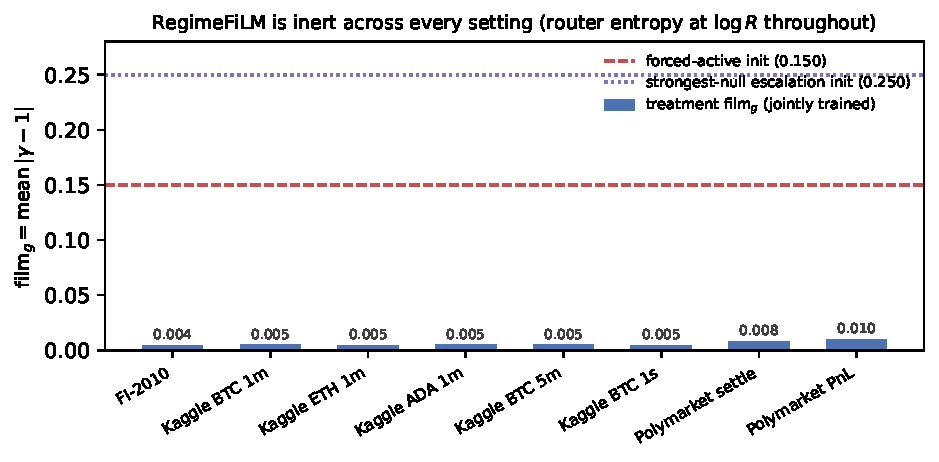
\includegraphics[width=0.78\linewidth]{figures/film_g_across_settings.pdf}
\caption{\textbf{RegimeFiLM is inert across every A/B setting.}  The
jointly-trained treatment $\mathrm{film}_g = \mathrm{mean}\,|\gamma-1|$
(bars) sits near $0.004$--$0.010$ on every dataset, asset, and
resolution---FI-2010, Kaggle BTC/ETH/ADA at three bar widths, and the two
Polymarket objectives---while a forced-active initialization starts at
$0.150$ and the strongest-null escalation at $0.250$ (dashed lines).  The
router entropy sits at its uniform maximum $\log R$ throughout.  The
modulation never grows from its exact identity initialization.}
\label{fig:film_across}
\end{figure}

% =============================================================================
% 4  GAUGE ABSORPTION
% =============================================================================
\section{Why Identity Is a Free Direction: Gauge Absorption}\label{sec:gauge}

\paragraph{The mechanism.}
The decay has a simple mechanistic explanation that also bounds the claim's
scope.  Our modulation is an \emph{input-side} affine,
$\tilde{x} = \gamma \odot \hat{x} + \beta$, applied to a block input that the
very next operations re-project (Eq.~\eqref{eq:selection}).  A constant
channel-wise scale folds \emph{exactly} into those projections as a
right-multiplied diagonal,
\begin{equation}\label{eq:fold}
  W_\bullet\,(\gamma\odot\hat x) = (W_\bullet\,\diag(\gamma))\,\hat x,
  \qquad \bullet\in\{\Delta,B,C\},
\end{equation}
and the shift folds into their biases, with \emph{no change} to the function
the block computes; the host weights can thus represent any constant
$(\gamma,\beta)$ themselves.  Identity is therefore a \emph{gauge}
direction---a flat, lossless valley the optimizer can slide along---so joint
training folds the modulation into the host weights and returns
$(\gamma,\beta)$ to $\mathbf{1},\mathbf{0}$, which is precisely the monotone
decay we observe.

\paragraph{The signature is the optimizer's, not the data's.}
Gauge absorption makes a sharp, falsifiable prediction: because the
absorption direction is a property of the \emph{block parameterization}, not
of the data, the decay rate should be the same across datasets.  It is.  The
predictability-supervised strongest-null escalation (forced-active FiLM,
router supervised directly on the efficiency-ratio bucket; load-balance term
\emph{disabled}) decays $\mathrm{film}_g$ monotonically at every logged step
on both datasets ($0.250 \to 0.144$ Kaggle, $0.250 \to 0.161$ FI-2010), with
$\mathrm{reg}_H \approx \log 4$ throughout---so the uniform router is not a
load-balance artifact.  An exponential fit $a\,e^{-t/\tau}+c$ matches both
trajectories at $R^2 > 0.999$ with near-identical parameters
($a \approx 0.30$, $\tau \approx 7000$ steps) and an asymptote $c \le 0$;
since $\mathrm{film}_g \ge 0$, the modulation provably converges to identity
rather than to a positive plateau.  That the decay rate is essentially
\emph{identical} across two very different markets points to the optimizer,
not the data, as the driver (Figure~\ref{fig:escalation_decay}).

\begin{figure}[t]
\centering
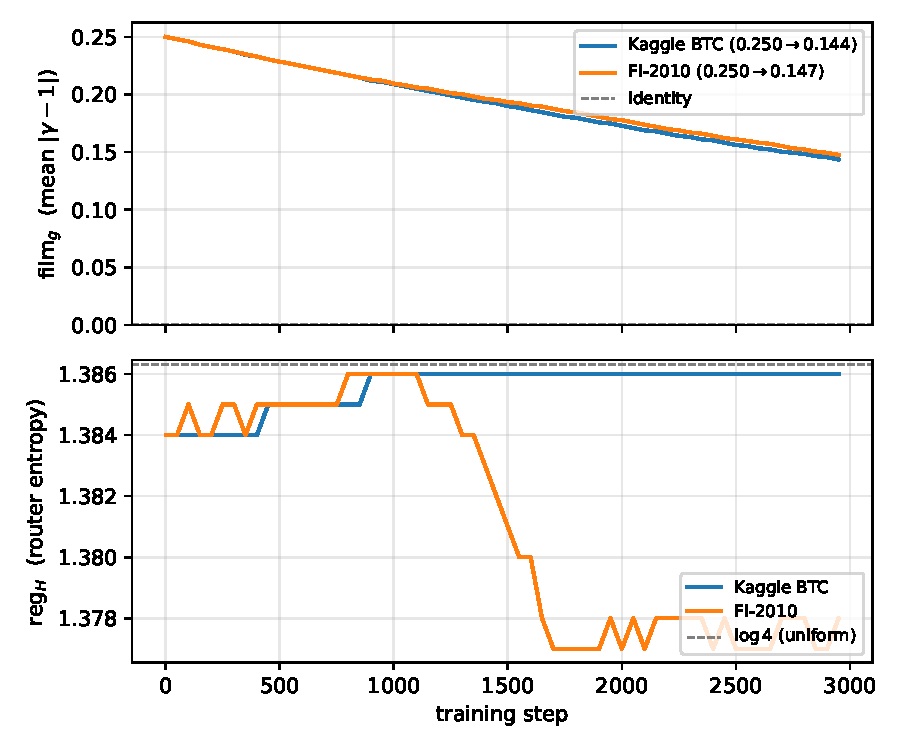
\includegraphics[width=0.60\linewidth]{figures/film_g_escalation_decay.pdf}
\caption{\textbf{Strongest-null test, and its placement-invariance.}  Forcing
the modulation active ($\mathrm{film}_g = 0.250$ at step~0) and supervising
the router directly on the efficiency-ratio bucket still decays
$\mathrm{film}_g$ monotonically toward identity on both datasets (top,
solid), with the router entropy $\mathrm{reg}_H$ pinned at its uniform
maximum $\log 4$ throughout (bottom).  An exponential fit gives
$R^2 > 0.999$ with a dataset-invariant time-constant $\tau \approx 7000$ and
an asymptote $\le 0$, so the modulation provably converges to identity.  The
\emph{post-scan} (output-side) gate (top, dotted) decays along the same
trajectory---its scale folds into the bias-free output projection just as the
input-side scale folds into $W_\Delta/W_B/W_C$---so the null is invariant to
where the affine is applied (Section~\ref{sec:overdetermined}).}
\label{fig:escalation_decay}
\end{figure}

\paragraph{Scope.}
This sharpens the result two ways.  First, it explains the dataset-invariant
decay constant: the absorption direction is a property of the
parameterization.  Second, it \emph{scopes} the null precisely.  Our claim is
that \emph{input-affine} conditioning of a selective scan is gauge-absorbable
and will not persist under joint training---not that regime conditioning is
impossible in principle.  Mechanisms outside this gauge---modulating
$W_\Delta/W_B/W_C$ directly inside the kernel, or otherwise conditioning a
quantity inserted \emph{between} the block's bounding projections---are not
trivially absorbable and are the natural next test.  An output-side gate,
which one might expect to qualify, does \emph{not}: its scale folds into the
block's output projection instead, as we show next.  Our contribution is the
negative that matters in practice: the most kernel-friendly, drop-in form of
the idea---the one that needs no change to the fused CUDA kernel---is exactly
the form the optimizer can and does undo.

% =============================================================================
% 5  OUTPUT-SIDE PLACEMENT: OVERDETERMINED
% =============================================================================
\section{An Output-Side Placement: the Null Is Overdetermined}
\label{sec:overdetermined}

The gauge argument names an obvious next test---gating \emph{after} the
scan---so we run it, under the \emph{identical} forced-active, ER-supervised
escalation, changing only where the learned $(\gamma,\beta)$ are applied.
Instead of the input-side $\tilde{x} = \gamma \odot \hat{x} + \beta$, we gate
the block \emph{output} $y' = \gamma \odot y + \beta$, the contribution the
block adds to the residual stream.  This placement does \emph{not} escape
absorption, and the reason is instructive.

\paragraph{The scale folds into the other face.}
Each Mamba-3 block ends in a \emph{bias-free} linear output projection,
$y = W_{\text{out}}\,h$, so a channel-wise output scale folds exactly into
it, $\gamma \odot (W_{\text{out}} h) = (\diag(\gamma)\,W_{\text{out}})\,h$---the
\emph{same} gauge move as the input side, now on the block's other face.

\paragraph{The shift is non-absorbable, and dies anyway.}
The additive shift $\beta$ is different: with no output bias to absorb it and
a nonlinear $\RMSNorm$ separating it from the next block's projections,
$\beta$ is genuinely \emph{non-absorbable}.  The escalation resolves both at
once.  Under forced activation and direct ER supervision, $\mathrm{film}_g$
\emph{and} $\mathrm{film}_b$ decay monotonically and in lockstep on both
datasets ($\mathrm{film}_g: 0.250 \!\to\! 0.147$ FI-2010,
$0.250 \!\to\! 0.143$ Kaggle; $\mathrm{film}_b$ tracks it within $0.005$),
with $\mathrm{reg}_H \approx \log 4$ throughout.  The exponential fit
$a\,e^{-t/\tau}+c$ gives the \emph{same} dataset-invariant signature as the
input-side gate---$a \approx 0.30$, $\tau \approx 7065$ (FI-2010) / $6598$
(Kaggle), asymptote $c \approx -0.05$, $R^2 > 0.999$---so the modulation
provably converges to identity here too.

\paragraph{Two mechanisms, no surviving direction.}
The null is therefore \emph{overdetermined} by two independent mechanisms.
Gauge absorption disposes of every direction the host weights can
represent---the multiplicative scale on \emph{either} face of the
block---which is why the decay constant is invariant to placement.
Reconstruction dominance disposes of the one direction they cannot: the
non-absorbable shift $\beta$, returned to identity at the same rate purely
because it earns nothing under the reconstruction objective.  A modulation
escaping both would have to act \emph{between} the block's bounding
projections---modulating $W_\Delta/W_B/W_C$ within the fused selective-scan
kernel---which is precisely the kernel-level change outside our hardware
envelope.  We thus delineate the boundary not as a parameterization that
survives training, but as the location---inside the kernel---a surviving
modulation would have to occupy, a boundary we demonstrate directly at toy
scale in Section~\ref{sec:synthetic}.

\paragraph{The regime is decodable yet unused---and not even needed.}
Two probes localize the failure.  A post-hoc reading of the
jointly-supervised router shows it is uniform \emph{per step} (per-sample
entropy $\approx \log 4$) with near-chance agreement against the
efficiency-ratio bucket ($0.25$--$0.31$ vs.\ $0.25$): direct supervision does
not even make the router regime-discriminative.  A frozen linear probe on the
unmodulated features decodes the per-step predictability bucket only weakly
($0.33$--$0.36$ vs.\ $0.25$ chance) and the volatility bucket somewhat better
($0.43$--$0.47$)---yet the volatility-axis gap is \emph{also} null.  Even on
the axis the representation encodes best, and even when the regime is supplied
by supervision, the in-scan modulation collapses to identity.

% =============================================================================
% 6  SYNTHETIC PROBE
% =============================================================================
\section{Elementary Small-Scale Probes}\label{sec:synthetic}

To show the absorption is the parameterization's and not an artifact of the
full LOB pipeline---and to turn the asserted in-kernel boundary into a
demonstrated one---we isolate the mechanism on a tiny selective scan run on the
pure-PyTorch \emph{reference} path (the slow path \texttt{mamba\_ssm} ships,
which the fused-kernel hardware limit does not touch), in seconds on the same
single 4080.

\paragraph{Folding: input-affine is absorbable, in-kernel is not.}
We place a forced-active modulation on a tiny reference-scan block and measure
whether it folds into primed host projections with no change in output.  The
input-affine scale folds \emph{exactly} (max output deviation
$1.2\times10^{-6}$): the recovered projections satisfy $W_\bullet^{\text{fit}}
\approx W_\bullet^{\text{base}}\,\diag(\gamma)$, the gauge move of
Eq.~\eqref{eq:fold}, at the level of round-off.  The \emph{same} modulation
applied to the projected $\Delta/\mathbf{B}/\mathbf{C}$ \emph{inside} the scan is
provably non-absorbable: the best-fit primed projection leaves a residual of
$1.3\times10^{-2}$, four orders of magnitude larger---a per-channel scale on the
post-softplus $\Delta$ cannot be matched by any linear reparameterization of the
pre-softplus projection.

\paragraph{Dynamics: the in-kernel placement survives.}
Under joint training (weight decay on) the forced-active input-affine modulation
decays to identity ($\mathrm{film}_g\!: 0.086 \to 0.010$), reproducing the LOB
null in miniature, while the non-absorbable in-kernel modulation \emph{persists}
($\mathrm{film}_g\!: 0.093 \to 0.175$, seeds 0--3): a modulation that lives
inside the kernel and survives the very training that decays the affine
form---the asserted boundary, demonstrated at toy scale.

\paragraph{Gauge vs.\ regularization.}
With weight decay \emph{off}, the input-affine modulation is no longer pulled to
identity ($0.086 \to 0.342$), and on the full model the same ablation flattens
the escalation decay: the exponential time constant lengthens from
$\tau\approx6685$ ($R^2=0.9999$) to $\tau\approx3\times10^{5}$ ($R^2=0.48$, no
clean decay), with $\mathrm{film}_g$ left at its forced-active initialisation.
So the decay along the gauge direction is driven by weight decay over a
\emph{flat} loss, not by the objective---distinguishing genuine gauge absorption
from a modulation that merely earns nothing.

\paragraph{A language-model control: the null is bounded by decodability.}
Because the collapse is optimizer-driven we check it is not specific to LOB data,
on the same single GPU: a 2-layer char-level Mamba LM on a two-domain corpus
(English prose vs.\ Python source), with the per-position regime inferred by a
context-aware router supervised on the domain and the \emph{same} input-affine
FiLM gating the second block.  Here the regime is \emph{strongly} decodable
(router ${\sim}0.95$ accuracy) and the FiLM does \emph{not} collapse:
$\mathrm{film}_g$ rises from $0.11$ to $0.52$.  Gauge absorption always removes
the constant component of the affine; the input-dependent component survives only
when the regime is decodable enough to be worth encoding.  In the
weakly-decodable LOB regimes the router collapses to uniform and the modulation
reduces to its absorbable constant part; a strongly-decodable regime engages
it---so the optimizer-driven collapse is the fate of \emph{weakly-decodable},
drop-in regime conditioning specifically.

% =============================================================================
% 7  THE SUBSTRATE IS NOT THE SUBJECT
% =============================================================================
\section{The Substrate Is Not the Subject}\label{sec:substrate}

The financial datasets are a demonstration substrate, chosen because genuine
non-stationarity is exactly the regime in which conditioning \emph{should}
help if anything does.  The full backbone is a Mamba-3 world model in the
DreamerV3/Drama lineage~\citep{hafner2023dreamerv3, wang2024drama,
lahoti2026mamba3}---a Transformer-over-depth LOB encoder with categorical
latents and a settlement auxiliary head---but none of that is the claim, and
we keep it to this paragraph.  Two checks confirm the substrate carries no
weight in the result.

\paragraph{No backbone dominates.}
A matched-parameter ablation ($\sim\!10.3$M params; held-out full-channel
Student-$t$ reconstruction NLL, lower is better) compares Mamba-1, Mamba-2,
Mamba-3 SISO, and a Mamba-3-matched pre-norm Transformer on FI-2010 and the
Kaggle BTC spot book.  No backbone leads on both datasets
(Table~\ref{tab:backbone_ablation}): Mamba-1 wins FI-2010 ($-0.5403$),
Mamba-2 wins Kaggle ($-0.0213$), Mamba-3 SISO is competitive
($-0.5346$/$0.0207$) but dominates neither, and a Mamba-3-matched pre-norm
Transformer ($-0.5041$/$0.0224$) is likewise competitive but non-dominant---so
the non-dominance is not an artifact of an under-tuned post-norm baseline.
This is exactly what a result about \emph{how} selective scans train, rather
than \emph{which} one is best, should predict.

\begin{table}[t]
\centering
\small
\begin{tabular}{lrrr}
\toprule
Backbone & Params & FI-2010 recon NLL & Kaggle recon NLL \\
\midrule
Mamba-1      & $11.45$M & $\mathbf{-0.5403}$ & $0.0241$ \\
Mamba-2      & $10.20$M & $-0.5309$ & $\mathbf{-0.0213}$ \\
Mamba-3 SISO & $10.30$M & $-0.5346$ & $0.0207$ \\
Transformer (pre-norm)  & $9.61$M  & $-0.5041$ & $0.0224$ \\
\bottomrule
\end{tabular}
\caption{Matched-parameter backbone ablation (held-out reconstruction NLL,
lower is better).  No backbone wins both datasets---Mamba-1 leads on FI-2010,
Mamba-2 on Kaggle---so the choice of sequence model is not the operative
variable.  A Mamba-3-matched (pre-norm, RMSNorm/SiLU/$4\times$ FFN)
Transformer is competitive but non-dominant.}
\label{tab:backbone_ablation}
\end{table}

\paragraph{Why SISO, and the hardware boundary.}
We run Mamba-3 SISO throughout because the MIMO kernel's dynamic
shared-memory footprint exceeds the RTX~4080 cap at every warp-valid
(rank, chunk) configuration---and the gating is not merely a 4080 artifact:
on an A100 the kernel runs only in a non-comparable compatibility path at
$\approx 9.5$\,s/iteration, and a configuration matched to our SISO state size
($d_{\text{state}}{=}128$) needs H100/H200/B200-class shared memory.  This is
the same boundary the gauge argument points at: the one place a surviving
modulation could live---inside the fused kernel---is the one place our small-scale
envelope cannot reach.  We report it as a scoping limitation, not a deferred
result.

\paragraph{The surviving economic edge is architecture-independent
(two-sentence coda).}
The same study yields one positive the architecture did \emph{not} carry: in
the high-predictability regime, a selective-participation \emph{strategy
gate}---a decision rule over the model's settlement signal, not an
architecture---turns a directionally-informative probability into a
survivable edge, with a market-block bootstrap over $127$ independent
held-out markets giving $\mathrm{P(profit)}{=}1.0$ and a $95\%$ CI of
$[{+}\$2{,}445,\,{+}\$7{,}747]$.  Crucially this edge is
\emph{architecture-independent}---a logistic regression on the same
spot-conditioned features reproduces and exceeds it ($+\$6{,}914$, vs.\ the
settlement head's $+\$5{,}147$ and a 3-seed EV-head mean of $+\$4{,}779$;
a direct-EV head additionally makes the marginal low-predictability regime
robust, $\mathrm{P(profit)}\,0.63\!\to\!0.98$--$0.99$, collapsing the regime
spread $6.2\times$ at comparable total PnL)---so the operative variable is the
features and the gate, not the sequence model, exactly as the null predicts.

% =============================================================================
% 8  DISCUSSION
% =============================================================================
\section{Discussion}\label{sec:discussion}

\paragraph{What the small scale bought.}
The $\le 1$-GPU constraint is why this study is conclusive rather than
suggestive.  An exact zero-initialized control is only meaningful if the
modulated and unmodulated runs are otherwise bit-identical, which is
cheap to guarantee at this scale and hard to audit at a large one.  The
forced-active escalations---deliberately fighting the optimizer with a
$50\times$ learning-rate router and direct supervision---are affordable
precisely because each run is small, so we could afford to lose, repeatedly,
on three datasets and an output-side variant until the mechanism was
overdetermined.  And the toy synthetic probe (Section~\ref{sec:synthetic})
that isolates the gauge runs in minutes.  None of these would change with
more compute: gauge absorption is a property of the block parameterization,
and the dataset-invariant $\tau$ is its fingerprint.

\paragraph{Takeaway for practitioners.}
If you want to condition a selective scan, do not gate its input (or its
output) with a learned affine and expect the modulation to persist---it is a
gauge the optimizer will remove, with a decay constant that does not depend
on your data.  The shift component survives the gauge argument but not
reconstruction dominance.  The only placements with a chance of surviving
joint training are \emph{inside} the bounding projections of the block,
acting on $W_\Delta/W_B/W_C$ within the fused kernel---which is exactly the
change that breaks drop-in, kernel-free deployment.  That trade-off, named
precisely, is the practical content of the null.

\paragraph{Limitations.}
Our claim is scoped to input/output-affine FiLM of a SISO selective scan
under reconstruction-dominated joint training; we do not test in-kernel
conditioning (outside our hardware), MIMO transitions, or non-affine
conditioning.  The economic coda is a deflated substrate result, not a
trading claim: it is a backtest with walk-the-book fills and is
architecture-independent by design.

\paragraph{Reproducibility and ethics.}
Every experiment runs on a single RTX~4080; matched YAML configurations for
Mamba-1/2/3 SISO and the matched Transformer reproduce the ablation with one
command per variant, and the escalation/exact-control protocol is released
with the code.  The work is a methodological diagnosis on public and
historical market data and makes no live-trading recommendation.

% =============================================================================
% REFERENCES
% =============================================================================
\bibliographystyle{plainnat}

\begin{thebibliography}{99}

\bibitem[Dao \& Gu(2024)]{dao2024mamba2}
T.~Dao and A.~Gu.
\newblock Transformers are {SSMs}: Generalized models and efficient algorithms through structured state space duality.
\newblock In \emph{Proc.\ ICML}, 2024.

\bibitem[Fedus et~al.(2022)]{fedus2022switch}
W.~Fedus, B.~Zoph, and N.~Shazeer.
\newblock Switch {T}ransformers: Scaling to trillion parameter models with simple and efficient sparsity.
\newblock \emph{JMLR}, 23:1--39, 2022.

\bibitem[Gu \& Dao(2024)]{gu2024mamba}
A.~Gu and T.~Dao.
\newblock Mamba: Linear-time sequence modeling with selective state spaces.
\newblock In \emph{Proc.\ COLM}, 2024.

\bibitem[Hafner et~al.(2023)]{hafner2023dreamerv3}
D.~Hafner, J.~Pasukonis, J.~Ba, and T.~Lillicrap.
\newblock Mastering diverse domains through world models.
\newblock \emph{arXiv preprint arXiv:2301.04104}, 2023.

\bibitem[Lahoti et~al.(2026)]{lahoti2026mamba3}
A.~Lahoti, K.~Y.~Li, B.~Chen, C.~Wang, A.~Bick, J.~Z.~Kolter, T.~Dao, and A.~Gu.
\newblock Mamba-3: Improved sequence modeling using state space principles.
\newblock In \emph{Proc.\ ICLR}, 2026 (arXiv:2603.15569).

\bibitem[Perez et~al.(2018)]{perez2018film}
E.~Perez, F.~Strub, H.~de~Vries, V.~Dumoulin, and A.~Courville.
\newblock {FiLM}: Visual reasoning with a general conditioning layer.
\newblock In \emph{Proc.\ AAAI}, 2018.

\bibitem[Wang et~al.(2024)]{wang2024drama}
W.~Wang et~al.
\newblock Drama: Mamba-enabled model-based reinforcement learning is sample and parameter efficient.
\newblock In \emph{Proc.\ ICLR}, 2025 (arXiv:2410.08893, 2024).

\bibitem[Zhang et~al.(2019)]{zhang2019deeplob}
Z.~Zhang, S.~Zohren, and S.~Roberts.
\newblock {DeepLOB}: Deep convolutional neural networks for limit order books.
\newblock \emph{IEEE Transactions on Signal Processing}, 67(11):3001--3012, 2019.

\end{thebibliography}

\end{document}
